\documentclass[border=4pt]{standalone}
\usepackage{tikz}
\usetikzlibrary{arrows.meta}
\begin{document}
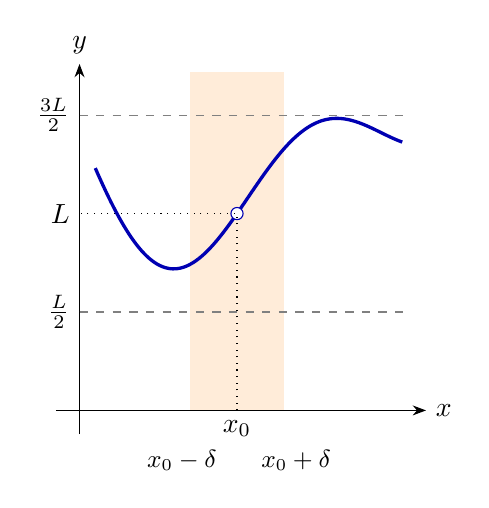
\begin{tikzpicture}[x=1cm,y=1cm,>=Stealth]
  \fill[orange!15] (1.4,0) rectangle (2.6,4.3);
  \draw[->] (-0.3,0) -- (4.4,0) node[right] {$x$};
  \draw[->] (0,-0.3) -- (0,4.4) node[above] {$y$};
  \draw[dashed,gray] (0,1.25) -- (4.2,1.25);
  \draw[dashed,gray] (0,3.75) -- (4.2,3.75);
  \node[left] at (0,2.5) {$L$};
  \node[left] at (0,1.25) {$\frac{L}{2}$};
  \node[left] at (0,3.75) {$\frac{3L}{2}$};
  \draw[very thick,blue!70!black,domain=0.2:4.1,samples=120]
       plot (\x,{2.5+0.9*sin(deg(1.6*(\x-2)))+0.25*(\x-2)*(\x-2)});
  \draw[blue!70!black,fill=white] (2,2.5) circle (2.2pt);
  \draw[dotted] (2,0) -- (2,2.5) -- (0,2.5);
  \node[below] at (2,0) {$x_0$};
  \node[below,yshift=-11pt] at (1.3,0) {\small $x_0-\delta$};
  \node[below,yshift=-11pt] at (2.75,0) {\small $x_0+\delta$};
\end{tikzpicture}
\end{document}
